\documentclass{article}%
\usepackage[T1]{fontenc}%
\usepackage[utf8]{inputenc}%
\usepackage{lmodern}%
\usepackage{textcomp}%
\usepackage{lastpage}%
\usepackage{authblk}%
\usepackage{graphicx}%
%
\title{The phosphatidylinositol{-}3 kinase I inhibitor BKM120 induces cell death in B{-}chronic lymphocytic leukemia cells in vitro}%
\author{Joshua Mosley}%
\affil{Institute of Bioinformatics and Biosignal Transduction, College of Bioscience and Biotechnology, National Cheng{-}Kung University, Tainan, Taiwan}%
\date{01{-}01{-}2012}%
%
\begin{document}%
\normalsize%
\maketitle%
\section{Abstract}%
\label{sec:Abstract}%
Researchers from Arizona State University and the University of Manchester are studying the way a colonisophage, or yellow blood stem cell type, delivers antibodies to cytoplasmic bacteria. They are the first scientists to directly observe the effects on the immune system of an isolated yellow blood type, not the normal types of antibodies produced by normal red blood cells.\newline%
"In an animal, the yellow blood type interacts with the bacteria that cause cancer in a controlled fashion," said Tatjana Muzic, PhD, a Ph.D. student at ASU. "Our study uncovered the mechanism that underlies this beneficial interaction and how it involves a specific antibody. This antibody functions as an integrator of the immune system proteins."\newline%
Synthetic antibodies are used to synthesize proteins, which can then act as synthetic antibodies or components, much like a spider is chemically engineered to manipulate the host proteins. The chemical structure and signal processing function of these synthetic antibodies is similar to a natural antibody, but they work in direct contrast. The alert antibodies deliver an antigen or message to the host cell, but the organelles communicate this by communicating information by sending an incoming wave of genetic material.\newline%
Researchers describe the chemistry and materials of the endotoxins (oxigenins) that produce the antibodies. First they keyed into a gene sequence, which determines how specific organic materials of the red blood cells are formed. They focused on an endotoxin present in yellow blood type, Eta1. This endotoxin initiates signaling that interferes with cell survival.\newline%
"In chickens, our red blood cells have been part of an overexpression of Eta1, which causes the red blood cells to grow white, while it also causes them to migrate back to the blood, which in turn initiates the cell's defense system against invading pathogens," Muzic said. "This disease causing behavior in red blood cells reveals the communication between Eta1 and the host{-}cell receptors on proteins called interleukin{-}10 (IL{-}10) proteins."\newline%
"We're showing that the endotoxins interact with the complex pathways responsible for physical and molecular differentiation that mediates the red blood cell formation and evolution," Muzic said. "We can identify the role Eta1 plays in the production of antibodies for all host{-} and disease{-}specific bacterial pathogens. These results can aid in designing the next generation of therapeutic agents for all pathogens."\newline%
These findings are supported by the Center for Science in Developmental Biology at the University of Manchester and the John Howard Society.\newline%
This research was also supported by the National Institutes of Health and the Mexican government's National Institute of Natural Production, financed by Lyon Pharma and S. Muzic et al.\newline%
More information about blood cell division biology can be found at http://www.bmc.org/Animal/BGH/MSN/0135681.html\newline%
Contact ID: NA{-}mmint@mail.ahu.edu

%
\subsection{Image Analysis}%
\label{subsec:ImageAnalysis}%


\begin{figure}[h!]%
\centering%
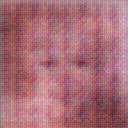
\includegraphics[width=150px]{500_fake_images/samples_5_357.png}%
\caption{A Close Up Of A Red And White Striped Tie}%
\end{figure}

%
\end{document}